\documentclass[pdf]{beamer}
\mode<presentation>{} 
\definecolor{Blue}{RGB}{0,0,100}
\usepackage{hyperref}
\usepackage{pgf}
\usepackage{tikz}
\usetikzlibrary{trees}
\usetikzlibrary{arrows,automata}
\usetikzlibrary{automata,positioning}
\usetikzlibrary{shapes}
\usepackage{tikz-qtree,tikz-qtree-compat}
\usepackage{mathtools,enumerate,amssymb}
\usepackage[utf8]{inputenc}
\usepackage[T1]{fontenc}
\usepackage[export]{adjustbox}
\usepackage{graphicx}
\usepackage{float}
\usepackage{mathptmx}
\usepackage{anyfontsize}
\usepackage{t1enc}
\usepackage{url}
\usepackage{lmodern}

\title{Introduction}
\subtitle{Human Computer Interaction}
\AtBeginSection[]{}

\setbeamertemplate{sidebar right}{}
\setbeamertemplate{footline}{%
\hfill\usebeamertemplate***{navigation symbols}
\hspace{1cm}\insertframenumber{}/\inserttotalframenumber}

\graphicspath{{./img/}}



\begin{document}

% Avram Constantin Dan
% Slide 1
\definecolor{myBlue}{RGB}{0,0,100}
\definecolor{background}{RGB}{255,255,255}

{\setbeamercolor{background canvas}{bg=background}
\begin{frame}
\vspace{10mm}
\huge{\raggedleft{\color{black}{\textbf{Introduction}}}}

\large{\raggedleft{\color{black} Human Computer Interaction}}

\begin{flushright}
\end{flushright}

\fontsize{7pt}{1pt}\selectfont{
Based on slide deck 

\textbf{Part 1. Introduction }

Human Computer Interaction I: Principles and Design

by

\textbf{Saul Greenberg}
\newline
Professor
\newline
\textbf{University of Calgary, Canada}
}

\textit{The new slides are marked with a *}

\fontsize{5pt}{1pt}\selectfont{ \textcolor{lightgray}
{Slide deck by Saul Greenberg. Permission is granted to use this for non-commercial purposes as long as general credit to Saul Greenberg is clearly maintained.
Warning: some material in this deck is used from other sources without permission. Credit to the original source is given if it is known.}}

\end{frame}}



% Inaintea codului fiecarui slide se vor scrie urmatoarele informatii:
% Nume si prenume student
% Numarul slide-ului corespunzator din prezentarea prof. Saul Greenberg
% Numele imaginilor inserate trebuie sa fie numar_slide_nume_imagine.extensie_imagine



% Avram Constantin Dan
% Slide 2

{\setbeamercolor{background canvas}{bg=background}
%\begin{frame}
%
%\vspace{8mm}
%\textcolor{myBlue}{\textbf{\Large{Administrivia}}}
%
%\textcolor{red}{\rule{10cm}{1mm}}
%
%\begin{figure}[h!]
%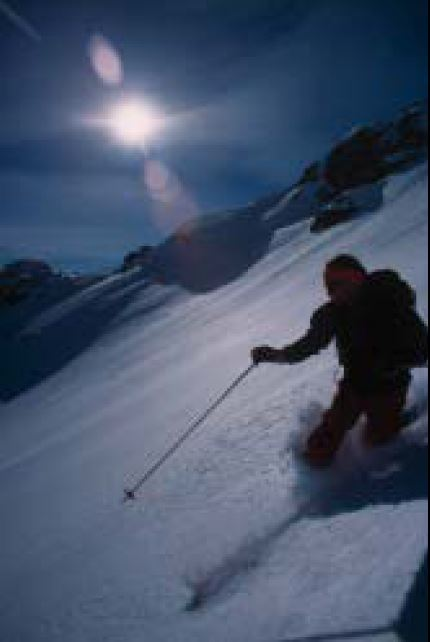
\includegraphics[width=35mm, height=50mm,right]{2_man_skiing.JPG}
%\end{figure}
%\vspace*{-60mm}
%\vspace{3mm}
%\textcolor{myBlue}{{\hspace{2mm}{Saul Greenberg}}}
%\begin{itemize}
%	\item[\textcolor{myBlue}{--}] \textcolor{myBlue}{{\small Human computer interaction}}
%    \item[\textcolor{myBlue}{--}] \textcolor{myBlue}{{\small Computer supported cooperative work}}
%\end{itemize}
%
%\vspace{3mm}
%\textcolor{myBlue}{{\hspace{2mm}{Contact information}}}
%\begin{itemize}
%	\item[\textcolor{myBlue}{--}] \textcolor{myBlue}{{\small saul@cpsc.ucalgary.ca}}
%    \item[\textcolor{myBlue}{--}] \textcolor{myBlue}{{\small 220-6087}}
%    \item[\textcolor{myBlue}{--}] \textcolor{myBlue}{{\small Math Sciences Building MS-680}}
%\end{itemize}
%
%\vspace{3mm}
%\textcolor{myBlue}{{\hspace{2mm}{Office hours}}}
%\begin{itemize}
%	\item[\textcolor{myBlue}{--}] \textcolor{myBlue}{{\small one hour before class on Monday and Wednesday}}
%    \item[\textcolor{myBlue}{--}] \textcolor{myBlue}{{\small by email any time}}
%    \item[\textcolor{myBlue}{--}] \textcolor{myBlue}{{\small by appointment: email or phone to arrange one}}
%    \item[\textcolor{myBlue}{--}] \textcolor{myBlue}{{\small drop in for urgent requests (but no guarantees!)}}
%\end{itemize}
%
%\begin{flushright}
%\fontsize{0.5pt}{1pt}\selectfont{ \textcolor{lightgray}
%{Saul Greenberg}}
%\end{flushright}
%\end{frame}}



{\setbeamercolor{background canvas}{bg=background}
\begin{frame}
\vspace{8mm}
\textcolor{myBlue}{\textbf{\Large{*Human Computer Interaction}}}

\textcolor{red}{\rule{10cm}{1mm}}

\centering
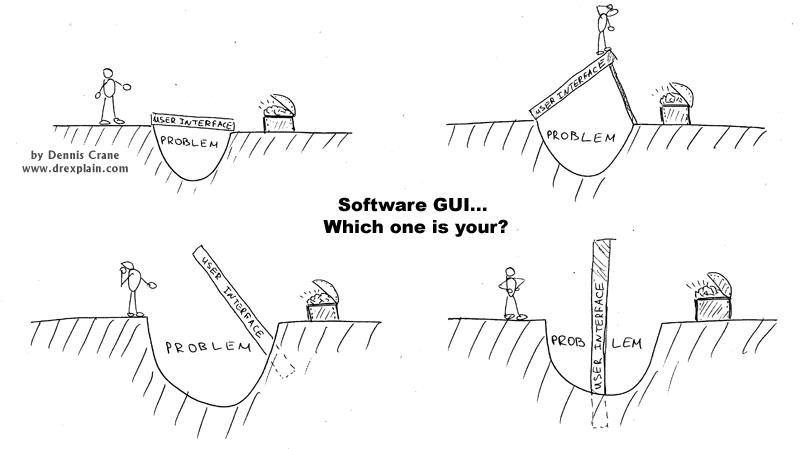
\includegraphics[scale=0.35]{0_motto.JPG}

\end{frame}}



% Avram Constantin Dan
% Slide 3

{\setbeamercolor{background canvas}{bg=background}
\begin{frame}
\vspace{8mm}
\textcolor{myBlue}{\textbf{\Large{Human Computer Interaction}}}

\textcolor{red}{\rule{10cm}{1mm}}

\centering
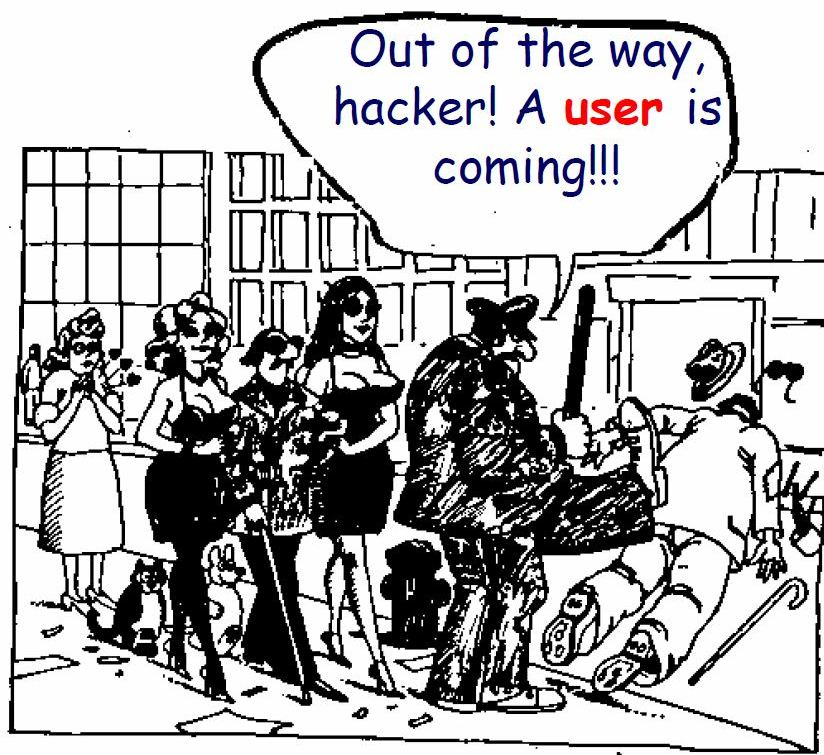
\includegraphics[scale=0.35]{3_out_of_the_way_hacker.JPG}

\end{frame}}



% Avram Constantin Dan
% Slide 4
{\setbeamercolor{background canvas}{bg=background}
\begin{frame}
\vspace{8mm}
\textcolor{myBlue}{\textbf{\Large{Moore's Law}}}

\textcolor{red}{\rule{10cm}{1mm}}

\begin{figure}
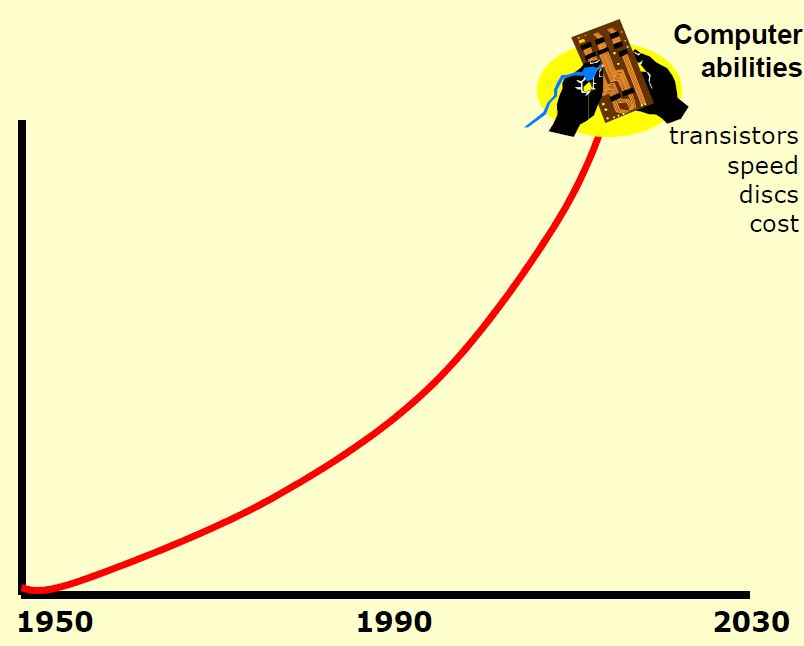
\includegraphics[width=80mm, height=70mm, center]{4_moores_law.JPG} \par
\end{figure}

\begin{flushright}
\fontsize{0.5pt}{1pt}\selectfont{ \textcolor{lightgray}
{Saul Greenberg}}
\end{flushright}

\end{frame}



% Avram Constantin Dan
% Slide 5
{\setbeamercolor{background canvas}{bg=background}
\begin{frame}
\vspace{8mm}
\textcolor{myBlue}{\textbf{\Large{Psychology}}}

\textcolor{red}{\rule{10cm}{1mm}}
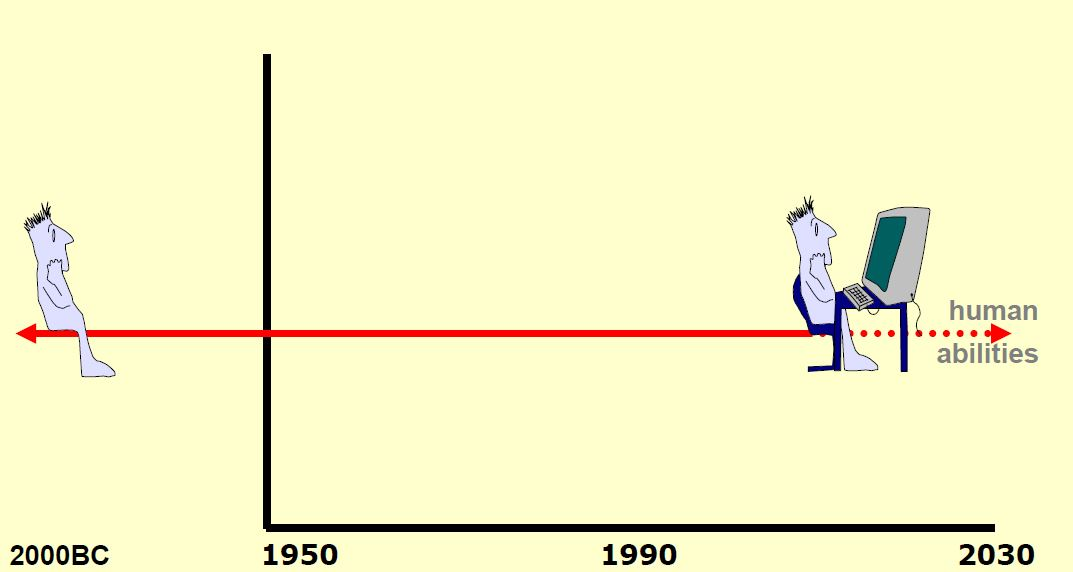
\includegraphics[width=110mm, height=70mm, left]{5_psychology.JPG} \par
\vspace{5mm}
\fontsize{0.5pt}{1pt}\selectfont{ \textcolor{lightgray}
{Slide idea by Bill Buxton}}
\vspace*{-4mm}
\begin{flushright}
\fontsize{0.5pt}{1pt}\selectfont{ \textcolor{lightgray}
{Saul Greenberg}}
\end{flushright}
\end{frame}



% Avram Constantin Dan
% Slide 6
{\setbeamercolor{background canvas}{bg=background}
\begin{frame}
\vspace{8mm}
\textcolor{myBlue}{\textbf{\Large{Where is the bottleneck?}}}

\textcolor{red}{\rule{10cm}{1mm}}
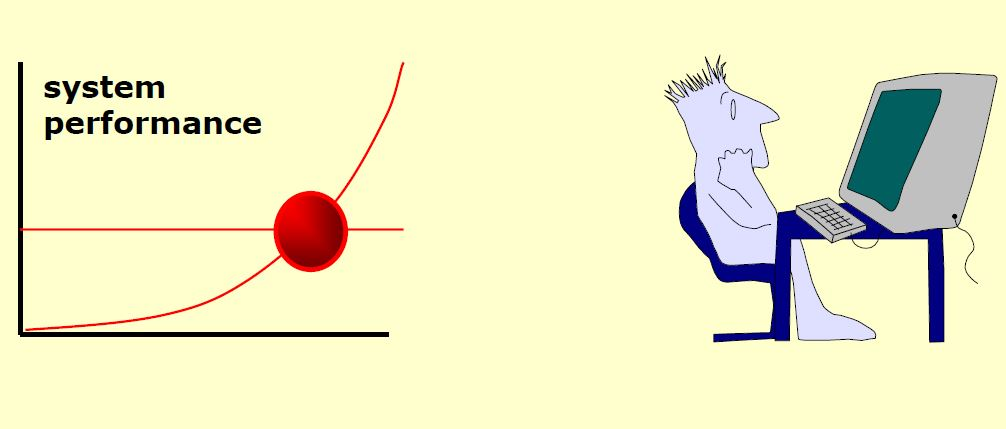
\includegraphics[width=110mm, height=60mm, left]{6_bottleneck.JPG} \par
\vspace{15mm}
\fontsize{0.5pt}{1pt}\selectfont{ \textcolor{lightgray}
{Slide idea by Bill Buxton}}

\vspace*{-4mm}
\begin{flushright}
\fontsize{0.5pt}{1pt}\selectfont{ \textcolor{lightgray}
{Saul Greenberg}}
\end{flushright}
\end{frame}



{\setbeamercolor{background canvas}{bg=background}
\begin{frame}
\vspace{8mm}
\textcolor{myBlue}{\textbf{\Large{*Definition of Human Computer Interaction}}}

\textcolor{red}{\rule{10cm}{1mm}}

Human-computer interaction is a discipline concerned with the design, evaluation and implementation of interactive computing systems for human use and with the study of major phenomena surrounding them.
\newline

\textbf{ACM SIGCHI Curricula for Human-Computer Interaction}


\end{frame}



% Avram Constantin Dan
% Slide 7
{\setbeamercolor{background canvas}{bg=background}
\begin{frame}
\vspace{8mm}
\textcolor{myBlue}{\textbf{\Large{Definition of Human Computer Interaction}}}
\textcolor{red}{\rule{10cm}{1mm}}
\vspace{5mm}
\newline
\textcolor{myBlue}{{\hspace{2mm}{A discipline concerned with the}}}
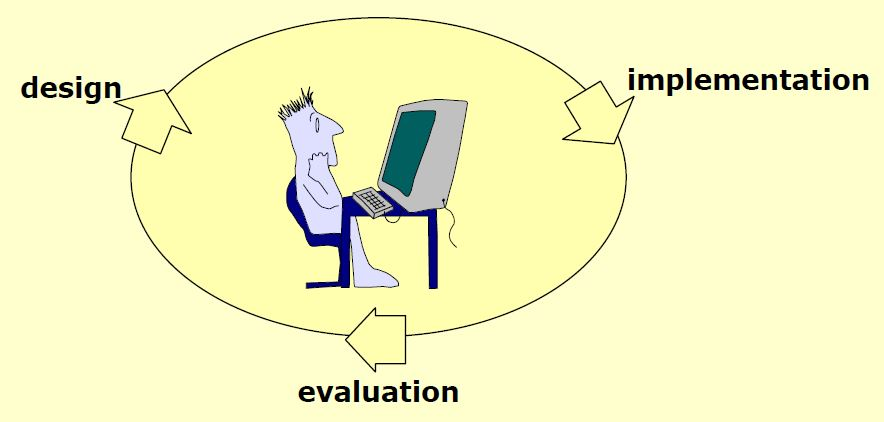
\includegraphics[width=110mm, height=50mm, left]{7_design_implementation.JPG} \par
\textcolor{myBlue}{{\hspace{2mm}{of interactive computing systems for human use}}}
\vspace{5mm}
\begin{flushright}
\fontsize{0.5pt}{1pt}\selectfont{ \textcolor{lightgray}
{Saul Greenberg}}
\end{flushright}
\end{frame}



{\setbeamercolor{background canvas}{bg=background}
\begin{frame}
\vspace{8mm}
\textcolor{myBlue}{\textbf{\Large{*Definition of Human Computer Interaction}}}

\textcolor{red}{\rule{10cm}{1mm}}

\begin{figure}
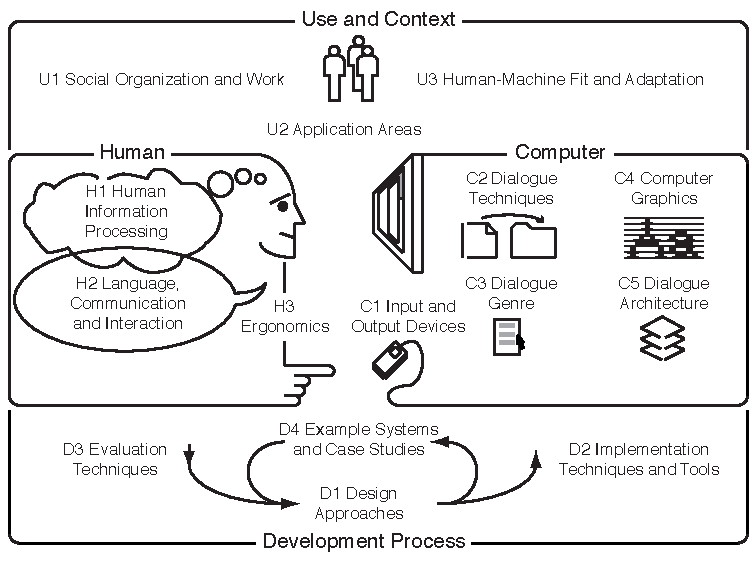
\includegraphics[scale=0.7, center]{figure_1.pdf}
\end{figure}

\textbf{ACM SIGCHI Curricula for Human-Computer Interaction}

\end{frame}



{\setbeamercolor{background canvas}{bg=background}
\begin{frame}
\vspace{8mm}
\textcolor{myBlue}{\textbf{\Large{*Human Computer Interaction}}}

\textcolor{red}{\rule{10cm}{1mm}}

The cardinal axiom of all user interface design:
\newline 

\textbf{A user interface is well-designed when the program behaves exactly how the user thought it would.}
\newline

\textbf{All the other rules of good UI design are just corollaries.}
\newline

Joel Spolsky, Controlling Your Environment Makes You Happy, Joel on Software

\url{https://www.joelonsoftware.com/2000/04/10/controlling-your-environment-makes-you-happy/}
\end{frame}}



%Ciugulea Alexandru-Sabin
%Slide 8
\begin{frame} 
\begin{center}
	{\textbf{\large An interface design process}}
\end{center}
\begin{figure}[h] \begin{flushright}
	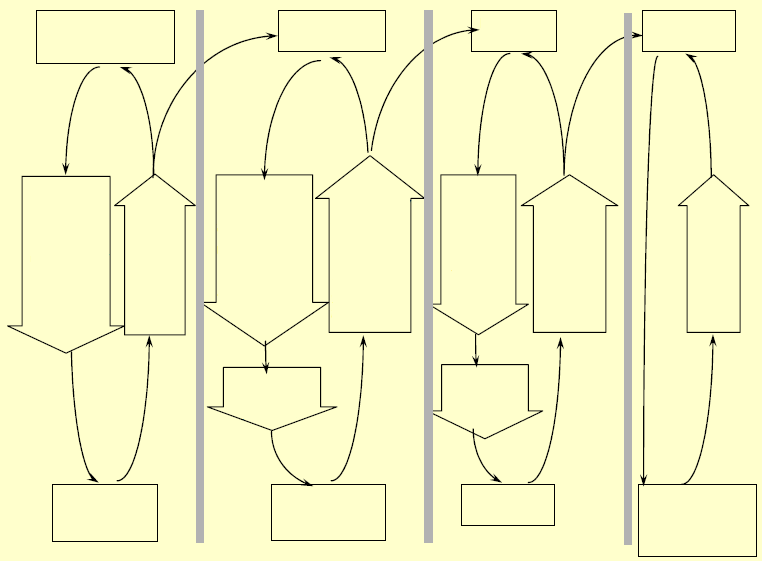
\includegraphics[width=0.98\textwidth]{11.png}
\end{flushright}
\end{figure}
\leavevmode\makebox(0,0){\put(-27,450){\selectfont{\textbf{\textit{\footnotesize Goals:}}}}}
\leavevmode\makebox(0,0){\put(-30,280){\selectfont{\textbf{\textit{\footnotesize Methods:}}}}}
\leavevmode\makebox(0,0){\put(-33,80){\selectfont{\textbf{\textit{\footnotesize Products:}}}}}
%prima coloana
\leavevmode\makebox(0,0){\put(11,468){\selectfont{\textbf{\tiny Articulate:}}}}
\leavevmode\makebox(0,0){\put(9,458){\selectfont{\textbf{\tiny -who users are}}}}
\leavevmode\makebox(0,0){\put(5,448){\selectfont{\textbf{\tiny -their key tasks }}}}
\leavevmode\makebox(0,0){\put(-3,332){\selectfont{\textnormal{\tiny Task }}}}
\leavevmode\makebox(0,0){\put(-7,320){\selectfont{\textnormal{\tiny centered }}}}
\leavevmode\makebox(0,0){\put(-10,307){\selectfont{\textnormal{\tiny system }}}}
\leavevmode\makebox(0,0){\put(-14,295){\selectfont{\textnormal{\tiny design }}}}
\leavevmode\makebox(0,0){\put(-23,275){\selectfont{\textnormal{\tiny Participatory }}}}
\leavevmode\makebox(0,0){\put(-20,265){\selectfont{\textnormal{\tiny design }}}}
\leavevmode\makebox(0,0){\put(-25,245){\selectfont{\textnormal{\tiny User- }}}}
\leavevmode\makebox(0,0){\put(-28,235){\selectfont{\textnormal{\tiny centered }}}}
\leavevmode\makebox(0,0){\put(-32,225){\selectfont{\textnormal{\tiny design }}}}
\leavevmode\makebox(0,0){\put(-27,80){\selectfont{\textbf{\tiny User and task }}}}
\leavevmode\makebox(0,0){\put(-26,70){\selectfont{\textbf{\tiny description }}}}
\leavevmode\makebox(0,0){\put(-7,280){\selectfont{\textit{\tiny Evaluate }}}}
\leavevmode\makebox(0,0){\put(-8,265){\selectfont{\textit{\tiny  }}}}
%a doua coloana
\leavevmode\makebox(0,0){\put(50,468){\selectfont{\textbf{\tiny Brainstorm }}}}
\leavevmode\makebox(0,0){\put(47,457){\selectfont{\textbf{\tiny design }}}}
\leavevmode\makebox(0,0){\put(15,330){\selectfont{\textnormal{\tiny Psychology of }}}}
\leavevmode\makebox(0,0){\put(12,320){\selectfont{\textnormal{\tiny everyday }}}}
\leavevmode\makebox(0,0){\put(8,310){\selectfont{\textnormal{\tiny things }}}}
\leavevmode\makebox(0,0){\put(5,285){\selectfont{\textnormal{\tiny User }}}}
\leavevmode\makebox(0,0){\put(2,275){\selectfont{\textnormal{\tiny involvement }}}}
\leavevmode\makebox(0,0){\put(-5,255){\selectfont{\textnormal{\tiny Representation }}}}
\leavevmode\makebox(0,0){\put(-4,245){\selectfont{\textnormal{\tiny metaphors }}}}
\leavevmode\makebox(0,0){\put(-5,180){\selectfont{\textnormal{\tiny low fidelity }}}}
\leavevmode\makebox(0,0){\put(-8,170){\selectfont{\textnormal{\tiny prototyping }}}}
\leavevmode\makebox(0,0){\put(-11,160){\selectfont{\textnormal{\tiny methods }}}}
\leavevmode\makebox(0,0){\put(5,90){\selectfont{\textbf{\tiny Throw-away }}}}
\leavevmode\makebox(0,0){\put(2,80){\selectfont{\textbf{\tiny paper }}}}
\leavevmode\makebox(0,0){\put(-1,70){\selectfont{\textbf{\tiny prototypes }}}}
\leavevmode\makebox(0,0){\put(13,320){\selectfont{\textit{\tiny Participatory }}}}
\leavevmode\makebox(0,0){\put(10,310){\selectfont{\textit{\tiny interaction }}}}
\leavevmode\makebox(0,0){\put(7,280){\selectfont{\textit{\tiny Task }}}}
\leavevmode\makebox(0,0){\put(5,270){\selectfont{\textit{\tiny scenario }}}}
\leavevmode\makebox(0,0){\put(1,260){\selectfont{\textit{\tiny walk- }}}}
\leavevmode\makebox(0,0){\put(-2,250){\selectfont{\textit{\tiny through }}}}
%a treia coloana
\leavevmode\makebox(0,0){\put(52,468){\selectfont{\textbf{\tiny Redefined }}}}
\leavevmode\makebox(0,0){\put(49,457){\selectfont{\textbf{\tiny designs }}}}
\leavevmode\makebox(0,0){\put(29,335){\selectfont{\textnormal{\tiny Graphical }}}}
\leavevmode\makebox(0,0){\put(26,325){\selectfont{\textnormal{\tiny screen }}}}
\leavevmode\makebox(0,0){\put(22,315){\selectfont{\textnormal{\tiny design }}}}
\leavevmode\makebox(0,0){\put(19,290){\selectfont{\textnormal{\tiny Interface }}}}
\leavevmode\makebox(0,0){\put(14,280){\selectfont{\textnormal{\tiny guidelines }}}}
\leavevmode\makebox(0,0){\put(13,260){\selectfont{\textnormal{\tiny Style }}}}
\leavevmode\makebox(0,0){\put(10,250){\selectfont{\textnormal{\tiny guides }}}}
\leavevmode\makebox(0,0){\put(3,180){\selectfont{\textnormal{\tiny high fidelity }}}}
\leavevmode\makebox(0,0){\put(0,170){\selectfont{\textnormal{\tiny prototyping }}}}
\leavevmode\makebox(0,0){\put(-1,160){\selectfont{\textnormal{\tiny methods }}}}
\leavevmode\makebox(0,0){\put(5,90){\selectfont{\textbf{\tiny Testable }}}}
\leavevmode\makebox(0,0){\put(2,80){\selectfont{\textbf{\tiny prototypes }}}}
\leavevmode\makebox(0,0){\put(23,320){\selectfont{\textit{\tiny Usability }}}}
\leavevmode\makebox(0,0){\put(20,310){\selectfont{\textit{\tiny testing }}}}
\leavevmode\makebox(0,0){\put(15,280){\selectfont{\textit{\tiny Heuristic }}}}
\leavevmode\makebox(0,0){\put(10,270){\selectfont{\textit{\tiny evaluation }}}}
%a patra coloana
\leavevmode\makebox(0,0){\put(53,468){\selectfont{\textbf{\tiny Completed }}}}
\leavevmode\makebox(0,0){\put(50,457){\selectfont{\textbf{\tiny designs }}}}
\leavevmode\makebox(0,0){\put(63,290){\selectfont{\textit{\tiny Field }}}}
\leavevmode\makebox(0,0){\put(58,280){\selectfont{\textit{\tiny testing }}}}
\leavevmode\makebox(0,0){\put(40,90){\selectfont{\textbf{\tiny Alpha/beta }}}}
\leavevmode\makebox(0,0){\put(36,80){\selectfont{\textbf{\tiny systems or }}}}
\leavevmode\makebox(0,0){\put(33,70){\selectfont{\textbf{\tiny complete }}}}
\leavevmode\makebox(0,0){\put(29,60){\selectfont{\textbf{\tiny specification }}}}
\end{frame}



%Ciugulea Alexandru-Sabin
%slide 9
{\setbeamercolor{background canvas}{bg=background}
\setbeamercolor{normal text}{fg=Blue}
\usebeamercolor[fg]{normal text}
\begin{frame}
	\vspace{8mm}
	\textcolor{Blue}{\textbf{\Large{Why an interface design process?}}}
    \textcolor{red}{\rule{10cm}{1mm}}
    
    \bigskip
    \textbf {63\% of large software projects go over cost}

    \begin{itemize}
    	\item[{--}] managers gave four usability-related reasons
        \begin{itemize}
        	\item[{$\bullet$}] users requested changes
            \item[{$\bullet$}] overlooked tasks
            \item[{$\bullet$}] users did not understand their own requirements 
            \item[{$\bullet$}] insufficient user-developer communication and understanding
     	\end{itemize}
   	\end{itemize}
     	\bigskip
     	\textbf {Usability engineering \textit{is} software engineering}
		\begin{itemize}
        \item[{--}] pay a little now, or pay a lot later! 
        \item[{--}] far too easy to jump into detailed design that is: 
        	\begin{itemize}
        	\item[{$\bullet$}] founded on incorrect requirements
          	\item[{$\bullet$}] has inappropriate dialogue flow
            \item[{$\bullet$}] is not easily used
         	\item[{$\bullet$}] is never tested until it is too late
        \end{itemize}
	\end{itemize}
    \bigskip
    \bigskip
     \begin{tikzpicture}[remember picture,overlay,shift={(current page.south east)}]
	\node[anchor=south east,xshift=0cm,yshift=2mm]{
\includegraphics[width=30mm, height=30mm]{18.png}};
\end{tikzpicture}
\end{frame}}



%Ciugulea Alexandru-Sabin
%slide 10

{\setbeamercolor{background canvas}{bg=background}
\setbeamercolor{normal text}{fg=Blue}
\usebeamercolor[fg]{normal text}
\begin{frame}
	\vspace{8mm}
	\textcolor{Blue}{\textbf{\Large{Foundations for designing interfaces}}}
    \textcolor{red}{\rule{10cm}{1mm}}
    
    \bigskip
    \textbf {Understanding users and their tasks}

    \begin{itemize}
    	\item[{--}] Task-centered system design
        \begin{itemize}
        	\item[{$\bullet$}] how to develop task examples
            \item[{$\bullet$}] how to evaluate designs through a task-centered walk-through
     	\end{itemize}
   	\end{itemize}
     	\bigskip
     	\textbf {Designing with the user}
		\begin{itemize}
        \item[{--}] User centered design and prototyping 
        \begin{itemize}
        	\item[{$\bullet$}] methods for designing with the user
          	\item[{$\bullet$}] low and medium fidelity prototyping
           
        \end{itemize}
        \item[{--}] Evaluating interfaces with users 
        	\begin{itemize}
        	\item[{$\bullet$}] the role of evaluation in interface designs
          	\item[{$\bullet$}] how to observe people using systems to

			detect interface problems
           
        \end{itemize}
	\end{itemize}
      \begin{tikzpicture}[remember picture,overlay,shift={(current page.south east)}]
	\node[anchor=south east,xshift=0cm,yshift=2mm]{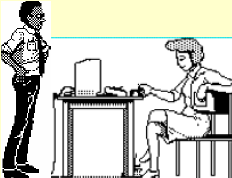
\includegraphics[width=30mm, height=25mm]{17.png}};
\end{tikzpicture}
\end{frame}}



%Ciugulea Alexandru-Sabin
%Slide 11

{\setbeamercolor{background canvas}{bg=background}
\setbeamercolor{normal text}{fg=Blue}
\usebeamercolor[fg]{normal text}
\begin{frame}
	\vspace{8mm}
	\textcolor{Blue}{\textbf{\Large{Foundations for designing interfaces}}}
    \textcolor{red}{\rule{10cm}{1mm}}
    
    \bigskip
    \textbf {Designing visual interfaces}

    \begin{itemize}
    	\item[{--}] Design of everyday things
        \begin{itemize}
        	\item[{$\bullet$}] what makes visual design work?
     	\end{itemize}
        \item[{--}] Beyond screen design
         \begin{itemize}
        	\item[{$\bullet$}] representations and metaphors
     	\end{itemize}
          \item[{--}] Graphical screen design
         \begin{itemize}
        	\item[{$\bullet$}] the placement of interface components on a screen
     	\end{itemize}
   	\end{itemize}
     	\bigskip
     	\textbf {Principles for design}
		\begin{itemize}
        \item[{--}] Design principles, guidelines, and usability heuristics 
        \begin{itemize}
        	\item[{$\bullet$}] using guidelines to design and discover usability problems
        \end{itemize}
	\end{itemize}
     \begin{tikzpicture}[remember picture,overlay,shift={(current page.south east)}]
	\node[anchor=south east,xshift=0cm,yshift=2mm]{
\includegraphics[width=17mm, height=22mm]{16.png}};
\end{tikzpicture}
\end{frame}}



%Ciugulea Alexandru-Sabin
%Slide 12
{\setbeamercolor{background canvas}{bg=background}
\setbeamercolor{normal text}{fg=Blue}
\usebeamercolor[fg]{normal text}
\begin{frame}
	\vspace{8mm}
	\textcolor{Blue}{\textbf{\Large{Objectives}}}
    \textcolor{red}{\rule{10cm}{1mm}}
 
    \bigskip
    \textbf {At the end of this course, you will know}
    \begin{itemize}
    \bigskip
    	\item[{--}] methods for grounding your design in reality
        \bigskip
        \item[{--}] methods for prototyping visual applications 
        \bigskip
        \item[{--}] methods for evaluating interface quality
        \bigskip
        \item[{--}] fundamentals of screen design and representations
        \bigskip
        \item[{--}] how to apply guidelines to interface designs
        \bigskip
        \item[{--}] how to apply your training in practice and continue your
education
	\end{itemize}
    \bigskip
       \begin{tikzpicture}[remember picture,overlay,shift={(current page.east)}]
	\node[anchor=east,xshift=0cm,yshift=2mm]{
\includegraphics[width=25mm, height=60mm]{15.png}};
\end{tikzpicture}
\end{frame}}



%Ciugulea Alexandru-Sabin
%Slide 13
{\setbeamercolor{background canvas}{bg=background}
\setbeamercolor{normal text}{fg=Blue}
\usebeamercolor[fg]{normal text}
\begin{frame}
	\vspace{8mm}
	\textcolor{Blue}{\textbf{\Large{How you will be evaluated}}}
    \textcolor{red}{\rule{10cm}{1mm}}
 
    \bigskip
    \textbf {Assignment 1}
    \begin{itemize}
    	\item[{--}] task centered design and prototyping (50\%/3)
    \end{itemize}
    \bigskip
    \textbf {Assignment 2}
    \begin{itemize}
        \item[{--}] usability evaluation of an existing system (50\%/3) 
    \end{itemize}
     \bigskip
    \textbf {Assignment 3}
    \begin{itemize}
        \item[{--}] system (re-)design, 

implementation 

and critique (50\%/3) 
    \end{itemize}
    \bigskip
    \bigskip
    \textbf {Exam (50\%)}
    \begin{tikzpicture}[remember picture,overlay,shift={(current page.south east)}]
	\node[anchor=south east,xshift=0cm,yshift=2mm]{
\includegraphics[width=55mm, height=35 	mm]{14.png}};
\end{tikzpicture}
    
    \textit {To pass the course}
    
	\textit	{one must pass the exam}
    
	\textit {and each of the assignments}
\end{frame}}



%Ciugulea Alexandru-Sabin
%Slide 14
{\setbeamercolor{background canvas}{bg=background}
\setbeamercolor{normal text}{fg=Blue}
\usebeamercolor[fg]{normal text}
\begin{frame}
	\vspace{8mm}
	\textcolor{Blue}{\textbf{\Large{Labs}}}
    \textcolor{red}{\rule{10cm}{1mm}}
 
    \bigskip
    \textbf {Critical to your success in assignments}
    \begin{itemize}
    	\item[{--}] elaboration of details
        \item[{--}] learn specific skills 
        \item[{--}] discuss intermediate results
        \item[{--}] class feedback on assignment 

milestones
	\end{itemize}
    \bigskip
    \bigskip
    \bigskip
    \bigskip
    \bigskip
    \bigskip
           \begin{tikzpicture}[remember picture,overlay,shift={(current page.south east)}]
	\node[anchor=south east,xshift=0cm,yshift=2mm]{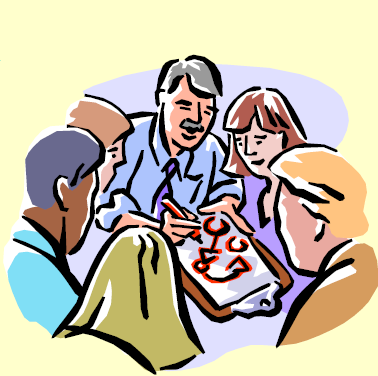
\includegraphics[width=50mm, height=50mm]{13.png}};
\end{tikzpicture}
    
\end{frame}}



{\setbeamercolor{background canvas}{bg=background}
\setbeamercolor{normal text}{fg=Blue}
\usebeamercolor[fg]{normal text}
\begin{frame}
	\vspace{8mm}
	\textcolor{Blue}{\textbf{\Large{*(G)UI Design versus (G)UI Development/Programming}}}
    \textcolor{red}{\rule{10cm}{1mm}}

\begin{itemize}
\item desktop GUI programming in C\#
\begin{itemize}
\item \textbf{Windows Forms}
\newline

\item \textbf{WPF} (Windows Presentation Foundation)
\begin{itemize}
\item  XAML based
\end{itemize}

\item \textbf{UWP} (Universal Windows Platform)
\begin{itemize}
\item  XAML based
\item  Windows 10 and Windows 10 Mobile
\end{itemize}
\end{itemize}

\item web GUI programming in C\#
\begin{itemize}
\item \textbf{ASP.NET Web Forms}
\newline

\item \textbf{ASP.NET MVC / ASP.NET Core MVC}

\end{itemize}
\end{itemize}

\end{frame}}



{\setbeamercolor{background canvas}{bg=background}
\setbeamercolor{normal text}{fg=Blue}
\usebeamercolor[fg]{normal text}
\begin{frame}
	\vspace{8mm}
	\textcolor{Blue}{\textbf{\Large{*(G)UI Design versus (G)UI Development/Programming}}}
    \textcolor{red}{\rule{10cm}{1mm}}

\begin{itemize}
\item GUI programming in Java
\begin{itemize}
\item \textbf{AWT API} (Abstract Windowing Toolkit) (mostly obsolete)
\newline

\item \textbf{Swing API}
\newline

\item \textbf{JavaFX} (meant to replace Swing)
\end{itemize}

\item Android UI programming
\end{itemize}

\end{frame}}



{\setbeamercolor{background canvas}{bg=background}
\setbeamercolor{normal text}{fg=Blue}
\usebeamercolor[fg]{normal text}
\begin{frame}
	\vspace{8mm}
	\textcolor{Blue}{\textbf{\Large{*(G)UI Builders}}}
    \textcolor{red}{\rule{10cm}{1mm}}

\begin{itemize}
\item Visual Studio 2017 \textbf{Windows Forms Designer}

\item Visual Studio 2017 \textbf{XAML Designer}

\item NetBeans GUI Builder (AWT/Swing)

\item Eclipse GUI Builder (Swing)

\item  Android Studio \textbf{Layout Editor}

\item ...

\end{itemize}

\end{frame}}



%Ciugulea Alexandru-Sabin
%Slide 15

{\setbeamercolor{background canvas}{bg=background}
\setbeamercolor{normal text}{fg=Blue}
\usebeamercolor[fg]{normal text}
\begin{frame}
	\vspace{8mm}
	\textcolor{Blue}{\textbf{\Large{*Bibliography}}}
    \textcolor{red}{\rule{10cm}{1mm}}

    \begin{itemize}
    	\item[] 
        \begin{itemize}
        	\item[{$\bullet$}] Saul Greenberg, \textbf{Introduction to Human Computer Interaction}, University of Calgary, Canada

        	\url{http://pages.cpsc.ucalgary.ca/~saul/481/}
        	
        	\item[{$\bullet$}] Keith Andrews, \textbf{Human Computer Interaction}, TU Graz, Austria

        	\url{https://courses.isds.tugraz.at/hci/}

        	\url{https://courses.isds.tugraz.at/hci/hci.pdf}
        	
        	\item[{$\bullet$}] ACM SIGCHI \textbf{Curricula for Human-Computer Interaction}
        	
        	\url{http://old.sigchi.org/cdg/index.html}
     	\end{itemize}
   	\end{itemize}

\begin{tikzpicture}[remember picture,overlay,shift={(current page.south east)}]
	\node[anchor=south east,xshift=0cm,yshift=2mm]{
\includegraphics[scale=0.4]{12.png}};
\end{tikzpicture}
\end{frame}}



{\setbeamercolor{background canvas}{bg=background}
\setbeamercolor{normal text}{fg=Blue}
\usebeamercolor[fg]{normal text}
\begin{frame}
	\vspace{8mm}
	\textcolor{Blue}{\textbf{\Large{*Bibliography}}}
    \textcolor{red}{\rule{10cm}{1mm}}

    \begin{itemize}
    	\item[] 
        \begin{itemize}
        	\item[{$\bullet$}] \textbf{Getting started with Windows Forms}

\url{https://docs.microsoft.com/en-us/dotnet/framework/winforms/getting-started-with-windows-forms}
        	
        	\item[{$\bullet$}] \textbf{Christian WPF Tutorial.net}

\url{http://www.wpftutorial.net/WPFIntroduction.html}
        	
        	\item[{$\bullet$}] \textbf{Getting Started with ASP.NET 4.5 Web Forms and Visual Studio 2017}

\url{https://docs.microsoft.com/en-us/aspnet/web-forms/overview/getting-started/getting-started-with-aspnet-45-web-forms/introduction-and-overview}

			\item[{$\bullet$}] \textbf{Getting started with ASP.NET MVC 5}

\url{https://docs.microsoft.com/en-us/aspnet/mvc/overview/getting-started/introduction/getting-started}
     	\end{itemize}
   	\end{itemize}
\end{frame}}



{\setbeamercolor{background canvas}{bg=background}
\setbeamercolor{normal text}{fg=Blue}
\usebeamercolor[fg]{normal text}
\begin{frame}
	\vspace{8mm}
	\textcolor{Blue}{\textbf{\Large{*Bibliography}}}
    \textcolor{red}{\rule{10cm}{1mm}}

    \begin{itemize}
    	\item[] 
        \begin{itemize}        	
        	\item[{$\bullet$}] \textbf{UI basics for Universal Windows Platform (UWP) apps}
        	
        	\url{https://msdn.microsoft.com/en-us/library/windows/apps/dn958432.aspx}
        	
        	\item[{$\bullet$}] \textbf{Java Programming Tutorial
Programming Graphical User Interface (GUI)}

\url{http://www.ntu.edu.sg/home/ehchua/programming/java/j4a_gui.html}

			\item[{$\bullet$}] \textbf{Create a UI by using XAML Designer in Visual Studio}

			\url{https://docs.microsoft.com/en-us/visualstudio/designers/creating-a-ui-by-using-xaml-designer-in-visual-studio?view=vs-2017}

			\item[{$\bullet$}] \textbf{C\# Windows Forms Application Tutorial with Example}

			\url{https://www.guru99.com/c-sharp-windows-forms-application.html}			
			
     	\end{itemize}
   	\end{itemize}
\end{frame}}



\end{document}